\documentclass[a4paper,12pt]{article}

\usepackage[utf8]{inputenc}
\usepackage{color,soul}
\usepackage{circledsteps}
\usepackage{ulem}
\usepackage{ragged2e}
\usepackage{blindtext}
\usepackage{hanging}
\usepackage{nopageno}
\usepackage[LGR,T1]{fontenc}
\usepackage[greek,english]{babel}
\usepackage{stix} %for caret
\usepackage[absolute]{textpos}
\usepackage{stackengine} %for multiple accents on one character
\usepackage{tikz}
\usepackage[paperwidth=5.5in, paperheight=19in, margin=0.7in]{geometry}
\usetikzlibrary{arrows.meta,decorations.pathreplacing,calligraphy,hobby}
\color{blue}
\setulcolor{blue}

\newcommand{\tickitem}{%
    \begin{tikzpicture}[remember picture,overlay]
        \draw[red] (-0.7, 0.1) -- (-0.6, 0) -- (-0.5, 0.5);
    \end{tikzpicture}%
}

\newcommand{\tickitemblue}{%
    \begin{tikzpicture}[remember picture,overlay]
        \draw[blue] (-0.7, 0.1) -- (-0.6, 0) -- (-0.5, 0.5);
    \end{tikzpicture}%
}
\newcommand{\crossitem}{%
    \begin{tikzpicture}[remember picture,overlay]
        \draw[red] (-0.9, 0) -- (-0.5, 0.4);
		\draw[red] (-0.9, 0.4) -- (-0.5, 0);
    \end{tikzpicture}%
}
\newcommand{\crosstickitem}{%
    \begin{tikzpicture}[remember picture,overlay]
		\draw[blue] (-1, 0.1) -- (-0.9, 0) -- (-0.5, 0.6);
		\draw[red] (-1, 0.4) -- (-0.5, 0);
    \end{tikzpicture}%
}
\newcommand{\thymusarrows}{%
    \begin{tikzpicture}[remember picture,overlay]
        \draw[->, red] (-1.7, 0.5) -- (-1, 0.3);
		\draw[->, red] (-0.5,1) -- (-0.5, 0.5);
    \end{tikzpicture}%
}
\newcommand{\multilinebrace}{
	
\begin{tikzpicture}[remember picture,overlay]
		\draw [pen colour ={red},
		decorate, 
		decoration = {calligraphic brace}
		] (-0.1,-0.3) -- (-0.1,0.2);
	\end{tikzpicture}
}

\newcommand{\downarrowabove}{
	\tiny
    \begin{tikzpicture}[remember picture,overlay]
        \node[] at (0.28,0.3) {$\downarrow$};
    \end{tikzpicture}
}

\newcommand{\curvedcircumflex}{
	\tikz[remember picture,overlay,hobby] 
	\draw plot coordinates {(0.05,0.25) (0.1,0.3) (0.15,0.25)};
}

\newcommand{\mediumlowtick}{
	\begin{tikzpicture}[remember picture,overlay]
		\draw (-0.1,0.3) -- (0,0);
		\draw (0,0) -- (4,2.5);
	\end{tikzpicture}
}

\newcommand{\leftofhorseline}{
	
\begin{tikzpicture}[remember picture,overlay]
		\draw (-0.1,0.7) -- (-0.4,-0.5);
	\end{tikzpicture}
}

\begin{document}
\begin{center}
Notes \& orig. drafts\\
\end{center}
\begin{flushright} 
\Circled{page 3}\\
\end{flushright}
\begin{center}
\ul{80 Flowers} - 
\setulcolor{red}
\ul{Epigraph} \hfill \color{red} 
\setulcolor{blue}
\ul{b. Dec 25/74}\\
\end{center}
\begin{flushleft}

\normalsize
\color{blue}
\begin{itemize}
\renewcommand{\labelitemi}{-}
\item \crosstickitem thyme pronounced time


\item \crossitem tread a measure - 

\normalsize
\item \tickitem bird(s) tread
\item \tickitem and grows by the {$\stackrel{\hbox{circles the rose}}{\hbox{rose tree(s)}}$} bud fire
\item \tickitem {[the Nine]} 
\color{red} 
\tiny
\stackengine{\stackgap}{heart us}{i.e.}{O}{l}
{\quietstack}{\useanchorwidth}{\stacktype} invisibly
\color{blue}
\normalsize
\item \tickitem gaping {$\stackrel{\hbox{bot. of}}{\hbox{pod}}$}  flower
\item \tickitem Pall\'adas: {$\stackrel{\hbox{\tiny{ochnay}}}{\hbox{\textgreek{Ὄχνη,}}}$}{$\stackrel{\hbox{\tiny{hand, skill of an artist}}}{\hbox{\textgreek{$\downarrowabove$χειρὸς εμ$\curvedcircumflex$ης}}}$}\\

%check accents for all Greek
{$\stackrel
	{\hbox
		{\tiny
			{sweet}
		}
	}
	{\hbox
		{\textgreek
			{γλυκερὸς
			}
		}
	}
$}
{$\stackrel
	{\hbox
		{\tiny
			{work - hard-work}
		}
	}
	{\hbox
		{\textgreek
		{πόνος
		}
		[ponus]
		}
	}
$}    

peartree my handiwork\par
(grafting the wild pear-tree (pyraster \textgreek{Αχρὰς})\par
in summer to $\stackrel{\hbox{fruit}}{\hbox{\sout{make}}}$ the upper stem\par
fragrant-\sout{fruited})
\item \tickitemblue as happens in 10 yrs
\item \tickitemblue N\stackon[-5pt]{\u{e}}{\'{}}p\u{e}ta
(\ul{catnip}
 \stackengine{\stackgap}{$\caretinsert$}{corruption of}{O}{c}
{\quietstack}{\useanchorwidth}{\stacktype} catmint)
 {$\stackrel
	{\hbox
		{\tiny
			{mint family ..}
		}
	}
	{\hbox
		{trailing .. gen.}
	}
$} \par
\tickitem aromatic* .. more or less hairy .. stem\sout{s} square\par
\tickitem .. leaves heart-shaped margins toothed ..\par
\tickitem blue or white flowers, often whorled close\par
\tickitem clusters on stems  $\caretinsert$ $\stackrel{\hbox{(or?) terminal spike}}{\hbox{.. corolla  2-lipped,}}$ 2-\par
upper, 3-lower joined at base, forming\par
narrow tube .. fruit a 2-celled capsule\par
\setulcolor{red}
which ri\ul{pe}ned splits into 4 parts\par
\setulcolor{blue}
L. Nepeta > Etrurian city .. /$\caretinsert$ $\stackrel{\hbox{species}}{\hbox{\ul{Nepeta}}}$\par
\tickitem \ul{cataria}, `tonic \& febrifuge' of Malabar\par
(SW India) coast, Nepenthe(s) epithet\par
\tickitem Egyptian drug > \ul{n\'e} \& \ul{penthos} sorrow\par
\tickitem Catnip .. ``man's \'earthly h\'ouseh\'old peac\'e''\par
\tickitem \& \ul{amaranth} `(unwithering)' $\stackrel{\hbox{persists}}{\hbox{\sout{persi}}}$ Whose\par
\tickitem nature (who's nature)'\par
%page has a few surprising apostrophes etc. I think they might be in red ink, so Z marking as he includes, but hard to say with image quality
\item \tickitem downland - {$\stackrel{\hbox{``loveth not to dance in}}{\hbox{quagmire(s)}}$}%sic unclosed
\item \tickitem sounds invisibly
\item \tickitem \textgreek{ἄρτος}  (Gk. bread) heart us 
%stacking below not quite right. poss better to have artos crossed out then superscript A&C bit
{$\stackrel
	{\hbox
		{\ul
		{A\&C} 
		III xiii 178
		}
	}
	{\hbox
		{\sout
		{artos} 
		}
	}
$} 
\end{itemize}
%down the lh margin
\begin{textblock*}{3.22in}(0.5cm,17.5cm)%
    \tiny
	\color{blue}
    \begin{minipage}{3.22in} 
		cf \ul{glecoma}\par
		(Gk. mint)\par
		\ul{hederacea}\par
		= ground ivy\par
		or gill-over-\par
		the-$\tickitem$ground\par
		or field balm\par
		flowers (clusters)\par
		light to dark\par
		blue\par
  \end{minipage}%
  \end{textblock*}%

\begin{textblock*}{3.22in}(0.5cm,22.5cm)%
	\tiny
	\color{blue}
	\begin{minipage}{3.22in} 
		\color{red}
		L.
		\color{blue} 
		\tickitem ripa - river\par
		bank, shore,\par
		seashore\par
		cf Plautus  re-\par
		breast\par
		feeding\par
	\end{minipage}%
\end{textblock*}%

\begin{textblock*}{3.22in}(0.5cm,25cm)%
	\tiny
	\begin{minipage}{3.22in} 
		\color{blue}
		L.
		\color{red}
		th\=us t\"us 
		\savestack{\greekequivalent}{\Longstack{gk \textgreek
		{τό
		}}}%
		\Longunderstack[r]{{\greekequivalent} \textgreek
		{θύος
		}}\par
		=incense\par
		frankincense\par
		\sout{fran}\par
	\end{minipage}%
\end{textblock*}%
% done as circled text but was the "therefore" (?) meant 
% to be included or excluded? 
\begin{textblock*}{3.22in}(0.5cm,26.7cm)%
	\tiny
	\begin{minipage}{3.22in} 
		\color{red}
		\Circled{
\stackengine{\stackgap}{therefore}{likely}{O}{l}
{\quietstack}{\useanchorwidth}{\stacktype}
\stackengine{\stackgap}{[thus]}{Gk toi}{O}{\stackalignment}
{\quietstack}{\useanchorwidth}{\stacktype}
}\par
\multilinebrace
mace =\par
nutmeg
	\end{minipage}%
\end{textblock*}%

\end{flushleft}

%arrows from serpyllum and century need to point to thymus
\begin{textblock*}{5cm}(6.3cm,4.5cm)%
\color{red}
\footnotesize
\begin{minipage}[t]{2cm}
variety:\par
T. serpyllum\par
\end{minipage}
\end{textblock*}%

\begin{textblock*}{5cm}(8.3cm,4cm)%
\color{red}
\footnotesize
\begin{flushright}
\begin{minipage}[t]{5cm}
\raggedleft
\setulcolor{red}
\ul{Century} - common\par
wild thyme Prov. E\par 
thymus \thymusarrows vulgaris sometimes\par
called horse-thyme\par
\end{minipage}
\end{flushright}
\end{textblock*}%

\begin{textblock*}{5cm}(6cm,6cm)%
\scriptsize
$\leftofhorseline$\savestack{\horsenote}{\Longstack{{``horse for single harness} {uncertain any .. concept(\sout{s}): }}}%
\Longunderstack[l]{{\horsenote} {\sout{firm} will $\color{red}\mediumlowtick$stand firm}} 
\end{textblock*}

\leavevmode
\\[0.5in]
\setlength{\parskip}{15pt}
% source references
\color{black}
\noindent\makebox[\linewidth]{\rule{\paperwidth}{0.4pt}}
\large
{\fontfamily{lmss}\selectfont
\setulcolor{black}
\begin{center}
\center\ul{Source references}
\end{center}
\normalsize
\begin{hangparas}{2em}{1}
	\textit{Century Dictionary} - defs for thyme, catnip, catmint, nepenthes\par
	Einstein - uncertain source (``horse for single harness'')\par
	\textit{Greek Anthology}, vol. III (Loeb, ed. W. R. Paton) - declamatory epigrams \#5, Palladas (4-5)\par
	Hudson, W. H., \textit{Nature in Downland} (quoting John Gerard on quagmires)\par
	\textit{A Latin Dictionary} (Lewis \& Short) - defs. for ripa and tūs, thūs\par
	Melville, \textit{Pierre} XXV, iv (386)\par
	Shakespeare, \textit{Antony and Cleopatra} - uncertain source\par
	\textit{Taylor's Encyclopedia of Gardening} - entries for Nepeta (792-793) and Glecoma (491)\par
\end{hangparas}
}

\end{document}

